En este capítulo damos algunas definiciones necesarias para presentar lo que
se conoce como descomposición de gráficas completas en thrackles. Este
es el principal problema que se trata en esta tesis.
Empezamos estableciendo conceptos relacionados con gráficas abstractas y después
hablaremos de gráficas en el plano, posteriormente explicamos el concepto de tipo de orden y cómo
se utiliza en este trabajo, continuamos hablando del anti-thickness abstracto
y del anti-thickness geométrico y finalmente explicamos el número cromático de una gráfica.

\section{Gráficas}
El concepto base del trabajo, del cual se desprenden otras definiciones, es el de gráfica.
Todas las definiciones que presentamos en esta sección fueron tomadas de~\cite{Chartrand2008}.

Una \emph{gráfica} $G$ está compuesta por un conjunto no vacío $V$ de objetos a los que llamamos \emph{vértices}
y por un conjunto $E$, de parejas de elementos de $V$, a los que llamamos \emph{aristas}. Denotamos
a la arista $e$ compuesta por los vértices $u$ y $v$ como $(u,v)$. Para describir a la gráfica $G$
compuesta por el conjunto $V$ de vértices y el conjunto $E$ de aristas escribimos $G=(V,E)$.
Para referirnos al conjunto de vértices de $G$ escribimos $V(G)$ y para referirnos
al conjunto de aristas de $G$ escribimos $E(G)$. En la figura~\ref{fig:g5vex} presentamos
un ejemplo de una gráfica.

\begin{figure}[t]
  \centering
  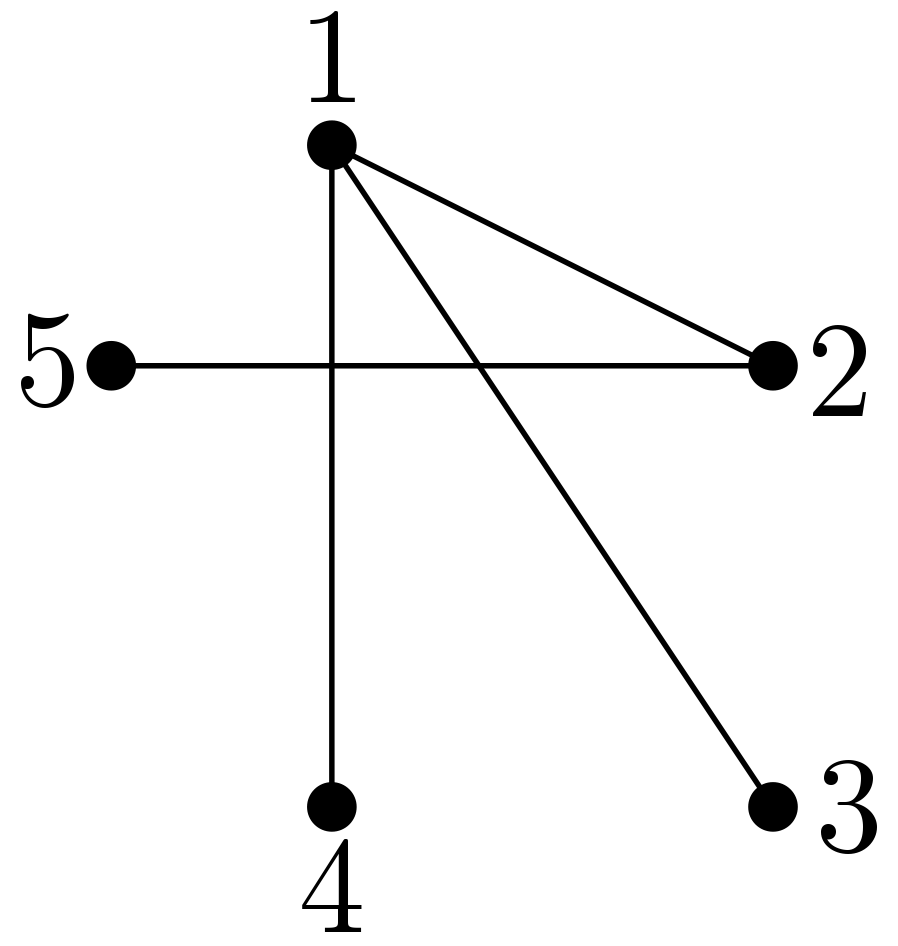
\includegraphics[width=0.27\linewidth]{g5vex.png}
  \caption{Una gráfica con cinco vértices y cuatro aristas. Los vértices $v_1$ y $v_2$
  son adyacentes y las aristas $(v_1,v_3)$ y $(v_1,v_4)$ son adyacentes.}
  \label{fig:g5vex}
\end{figure}
% \begin{figure}[htb]
%   \centering
%   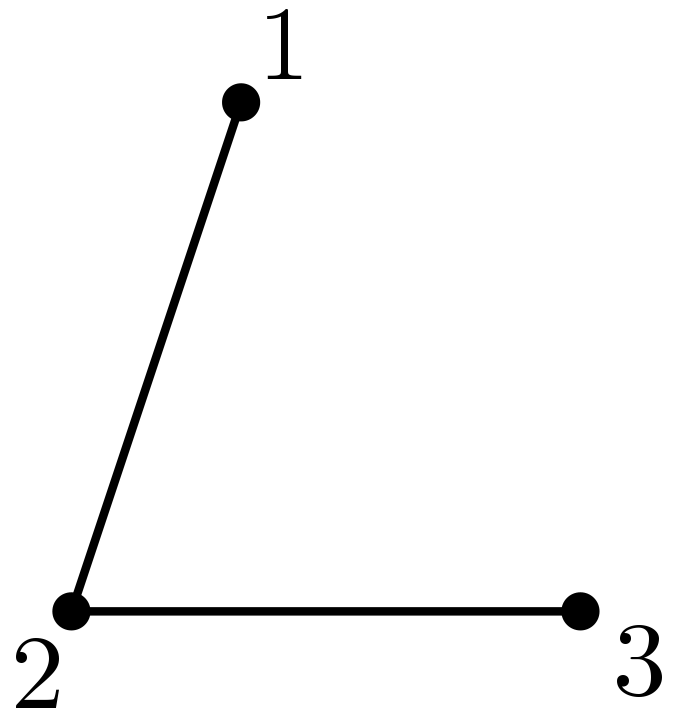
\includegraphics[width=0.3\linewidth]{exady}
%   \caption{En esta gráfica el vértice $1$ es adyacente con el vértice $2$ pero
%   no es adyacente con el vértice $3$.}
%   \label{fig:exady}
% \end{figure}
Decimos que \emph{dos vértices $u,v\in V(G)$ son adyacentes} si existe la arista
$(u,v)\in E(G)$. Decimos que \emph{dos aristas $e_1,e_2 \in E(G)$ son adyacentes}
si inciden en el mismo vértice. La figura~\ref{fig:g5vex} ilustra
un ejemplo de estos conceptos.
Una gráfica es \emph{completa} si cada pareja de vértices
en la gráfica es adyacente. Mostramos un ejemplo de adyacencia de
aristas en la figura~\ref{fig:g5vex} y un ejemplo de una gráfica completa en la figura~\ref{fig:excomplete}.
Para denotar una gráfica completa con $n$
vértices escribimos $K_n$. Una gráfica $G$ es \emph{bipartita} si es posible
dar una partición\footnote{Una partición $P$ de un conjunto $X$ es
una colección de subconjuntos que cumplen lo siguiente:
\begin{itemize}
\item Ningún elemento de $P$ es el conjunto vacío.
\item La unión de todos los elementos de $P$ es exactamente el conjunto $X$.
\item La intersección de cualesquiera dos elementos de $P$ es vacía.
\end{itemize} }
de $V(G)$ en dos subconjuntos $U$ y $W$ de tal manera que cada
arista de $G$ tenga un extremo en $U$ y otro extremo en $W$. Presentamos
un ejemplo de gráfica bipartita en la figura~\ref{fig:exbipar}.
\begin{figure}[htb]
  \centering
  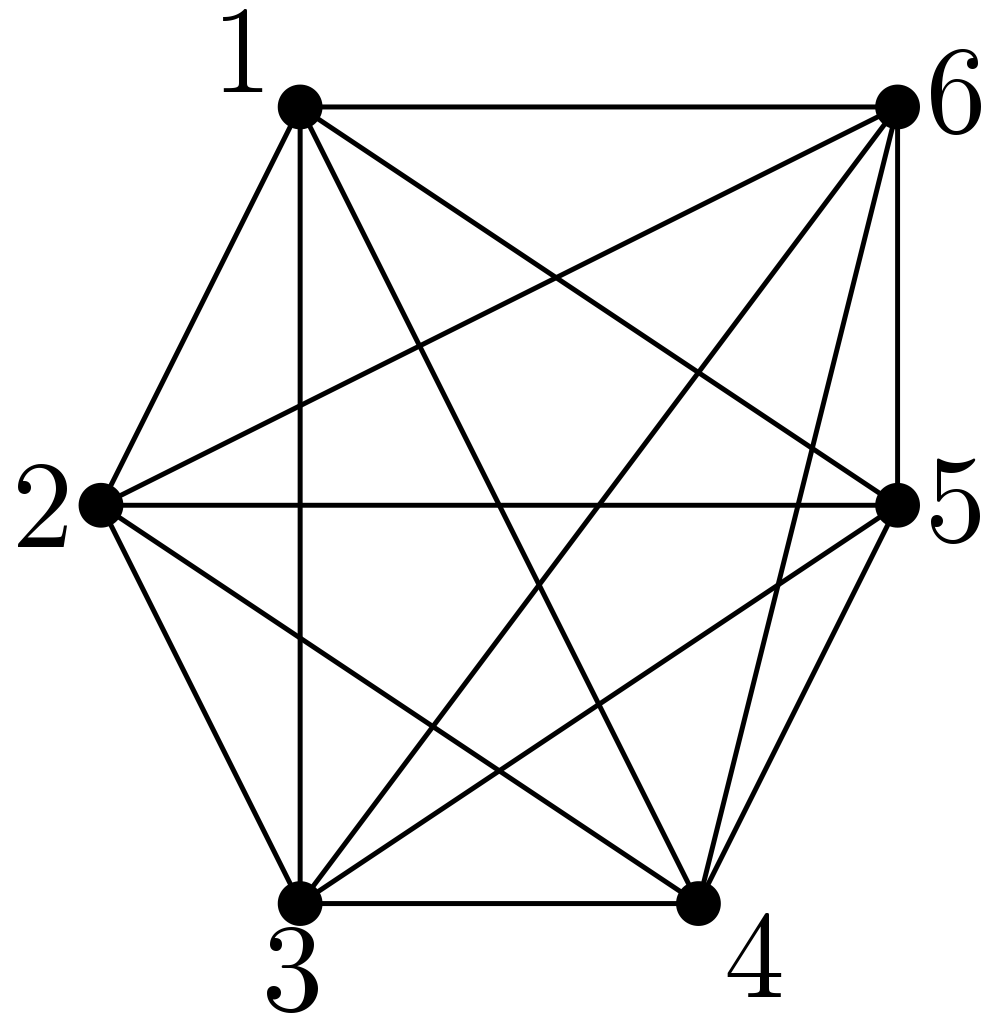
\includegraphics[width=.4\linewidth]{excomplete}
  \caption{La gráfica completa con 6 vértices tiene una arista por cada par de vértices.}
  \label{fig:excomplete}
\end{figure}
\begin{figure}[h]
  \centering
  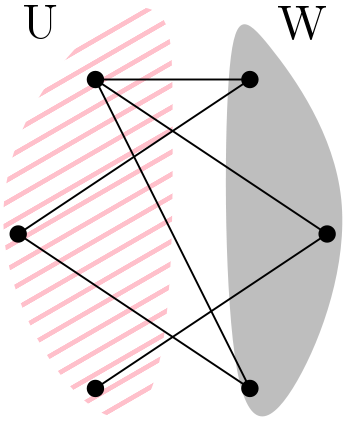
\includegraphics[width=0.3\linewidth]{exbipartita}
  \caption{Un ejemplo de una gráfica bipartita con bipartición $U, W$, ambos conjuntos son de tamaño tres.}
  \label{fig:exbipar}
\end{figure}

Una \emph{descomposición} $\mathcal{D}$ de una gráfica $G$ es una colección
$\mathcal{D}=\{G_1,G_2,\dots,G_k\}$ de subgráficas de $G$, que cumple con dos
condiciones:
\begin{enumerate}
  \item Ninguna subgráfica $G_i$ contiene vértices aislados.
  \item Cada arista de $G$ pertenece a exactamente una subráfica $G_i$ de
  $\mathcal{D}$.
\end{enumerate}
En este trabajo decimos que una gráfica $G$ cubre a una arista $e$ si sucede
que $e\in E(G)$.

Nótese que, en otras palabras, las subgráficas de la colección son disjuntas en
aristas y su unión cubre a $E(G)$.
La figura~\ref{fig:exdecom} ilustra un ejemplo de una descomposición de la
gráfica $K_4$.
\begin{figure}[htbp]
  \centering
  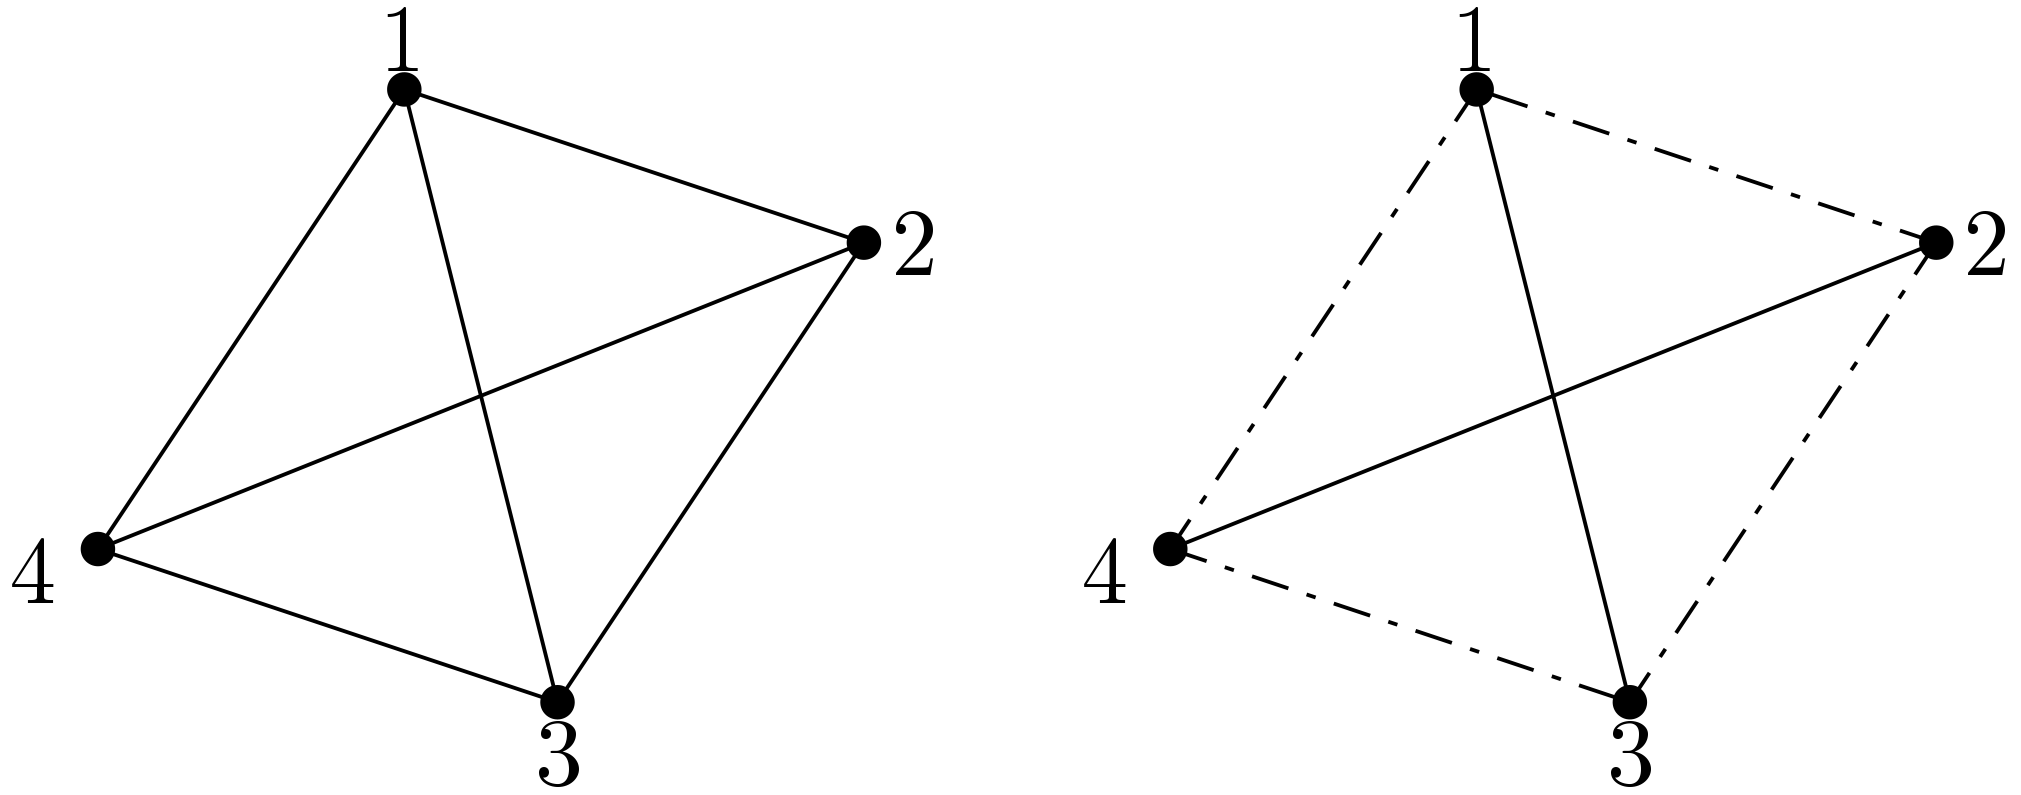
\includegraphics[width=0.8\linewidth]{exdecom}
  \caption{Un ejemplo de una descomposición $\mathcal{D}$ de $K_4$ en dos
  gráficas. Aquí $\mathcal{D}=\{G_1,G_2\}$ donde $G_1$ es la gráfica inducida
  por las aristas $(v_1,v_4),(v_1,v_2),(v_2,v_3),(v_3,v_4)$ y
  $G_2$ es la gráfica inducida por las aristas $(v_1,v_3),(v_2,v_4)$.}
  \label{fig:exdecom}
\end{figure}
%
% Introducir la próxima sección
%

En este trabajo hacemos descomposiciones de dibujos de gráficas (abstractas) en
gráficas geométricas que cumplen con cierta propiedad, que explicamos más
adelante. En la siguiente sección exponemos el concepto de dibujo de una
gráfica y de gráfica geométrica.

\subsection{Gráfica geométrica}
En esta sección abordamos uno de los conceptos clave de este trabajo,que son
las gráficas geométricas. Empezamos explicando el concepto de un
\emph{dibujo} de una gráfica (abstracta), para continuar con la descripción
de un dibujo de una gráfica, con características especiales, al que llamamos
\emph{gráfica geométrica}.

Los primeros dos párrafos de esta sección fueron tomados de~\cite{Pach2013}. El
tercer párrafo fue extraído de~\cite{Lara2019}. El cuarto párrafo fue tomado
de~\cite{Pach2011}.

Un \emph{dibujo} $\mathsf{G}=(\mathsf{V},\mathsf{E})$ de una gráfica $G$ es una
representación de la gráfica $G$ en el plano tal que 1) cada vértice de $G$ es
representado por un punto en el plano y 2) cada arista de $G$ es representada
como una curva simple continua que conecta un par de puntos. El conjunto de
vértices $\mathsf{V}$ y el conjunto de aristas $\mathsf{E}$ de $\mathsf{G}$
son los puntos y las curvas, respectivamente. Sin perdida de generalidad nos
referimos al conjunto de puntos de $\mathsf{G}$ como $V(\mathsf{G})$, y les
llamamos vértices, y nos referimos al conjunto de curvas de $\mathsf{G}$ como
$E(\mathsf{G})$, y les llamamos aristas.

Cuando restringimos las curvas que representan a las aristas del dibujo de $G$
a segmentos de recta, llamamos al dibujo de la gráfica \emph{gráfica
geométrica}. Una gráfica geométrica es completa si existe un segmento de recta
entre cada par de vértices de $V(\mathsf{G})$. En la figura~\ref{fig:exdrawk5}
mostramos un dibujo de $K_5$ y una gráfica geométrica de $K_5$. Sea $S$ un
conjunto de $n$ puntos en posición general en el plano y sea $\mathsf{G}$
una gráfica geométrica de $G$. Decimos que $\mathsf{G}$ está definida sobre $S$
si $V(\mathsf{G}) = S$. Cualquier conjunto $S$ de puntos en posición general
induce una gráfica geométrica completa.

\begin{figure}[htpb]
  \centering
  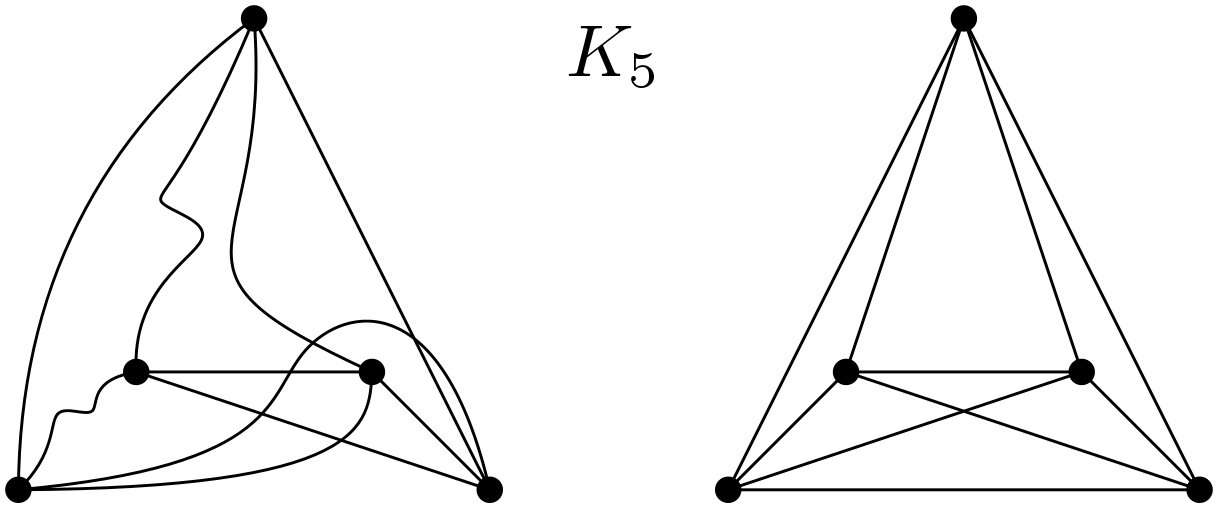
\includegraphics[width=0.5\linewidth]{exdrawk5}
  \caption{A la izquierda observamos un dibujo de $K_5$ y a la derecha
  observamos una gráfica geométrica de $K_5$.}
  \label{fig:exdrawk5}
\end{figure}

Todos los conceptos definidos para gráficas (abstractas) han sido heredados de
manera natural para los dibujos de gráficas, sin embargo, como la gráfica
geométrica está definida en el plano, es necesario redefinir el concepto de
adyacencia de aristas. Decimos que dos aristas $e_1,e_2 \in E(\mathsf{G})$ se
\emph{cruzan} si existe un punto $p$, en alguna de las aristas, tal que en $p$
la arista $e_1$ pasa de un lado de la arista $e_2$ hacia el otro lado. Decimos
que dos aristas $e_1, e_2 \in E(\mathsf{G})$ son \emph{adyacentes} si comparten
un vértice. En este trabajo decimos que dos aristas de una gráfica geométrica se
\emph{intersectan} si son adyacentes o si se cruzan.
Mostramos un ejemplo de intersección de aristas en la
figura~\ref{fig:exintersection}.
\begin{figure}[htpb]
  \centering
  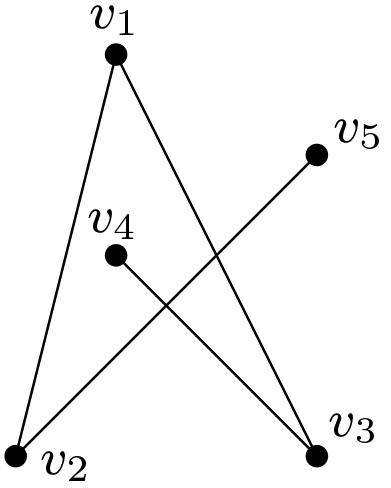
\includegraphics[width=0.2\linewidth]{exintersection}
  \caption{En este ejemplo la arista $(v_1,v_2)$ no se intersecta con la arista
  $(v_3,v_4)$ (son disjuntas) pero sí se intersecta con la arista $(v_2,v_5)$.
  La arista $(v_2,v_5)$ se cruza con la arista $(v_3,v_4)$ y por lo tanto se
  intersectan.}
  \label{fig:exintersection}
\end{figure}
% Sin perdida de generalidad
% representamos a una gráfica geométrica como $\mathsf{G}$ y nos referimos a su
% conjunto de vértices como $V(\mathsf{G})$ y a su conjunto de aristas como
% $E(\mathsf{G})$.

El concepto que estudiamos en esta tesis está relacionado con gráficas
geométricas donde cada par de aristas se intersectan una vez, estas gráficas
geométricas reciben el nombre de thrackles. En la siguiente sección explicamos
formalmente qué son los thrackles.

\subsection{Thrackles} \label{seccion_thrackles}
Sea $\mathsf{G}$ un dibujo de una gráfica $G$. Decimos que $\mathsf{G}$ es un
\emph{thrackle} si cada par de aristas se intersecta exactamente una vez. La
figura~\ref{fig:exmaxth} ilustra un ejemplo de thrackle.
Los thrackles fueron definidos por John Conway en la década de
1960~(\cite{Pach2013}). Conway también conjeturó que el número de aristas en un
thrackle no puede exceder el número de sus vértices~(\cite{Fulek2011}).
Un thrackle de $n$ vértices es \emph{máximo} si tiene exactamente
$n$ aristas. La figura~\ref{fig:exmaxth} muestra un thrackle máximo.

\begin{figure}[htpb]
  \centering
  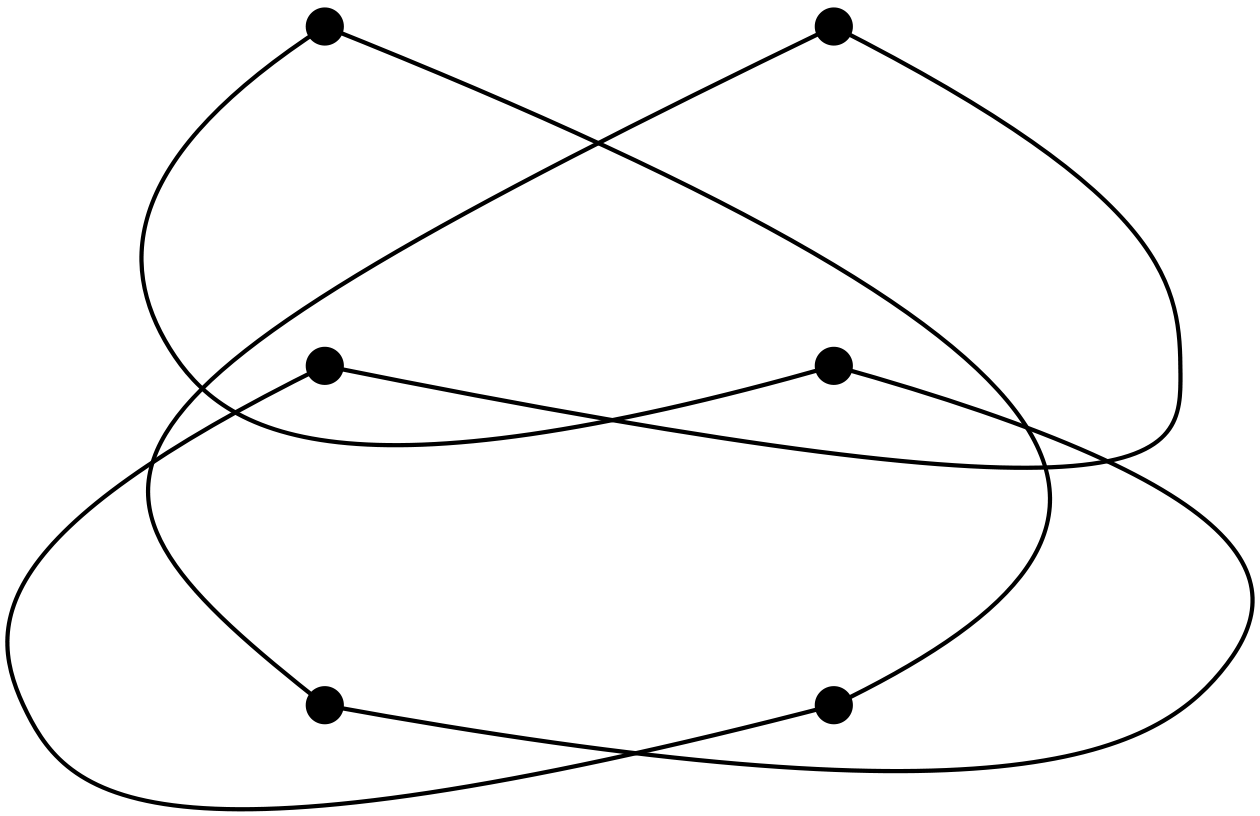
\includegraphics[width=0.45\linewidth]{exmaxth}
  \caption{Un thrackle máximo sobre un conjunto de seis vértices.}
  \label{fig:exmaxth}
\end{figure}

\begin{figure}[htb]
  \centering
\begin{subfigure}[h]{.4\textwidth}
  \centering
  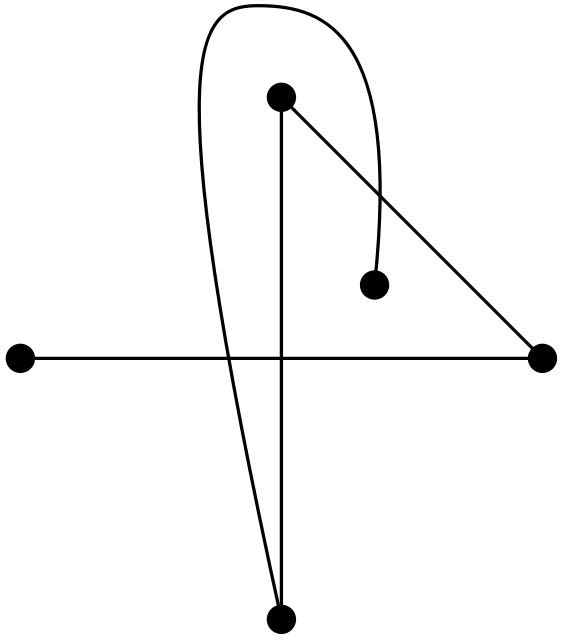
\includegraphics[width=.6\linewidth]{exthtop}
  \caption{Un thrackle con cinco vértices.}
  \label{fig:exthtop}
\end{subfigure}\hfill%
\begin{subfigure}[h]{.4\textwidth}
  \centering
  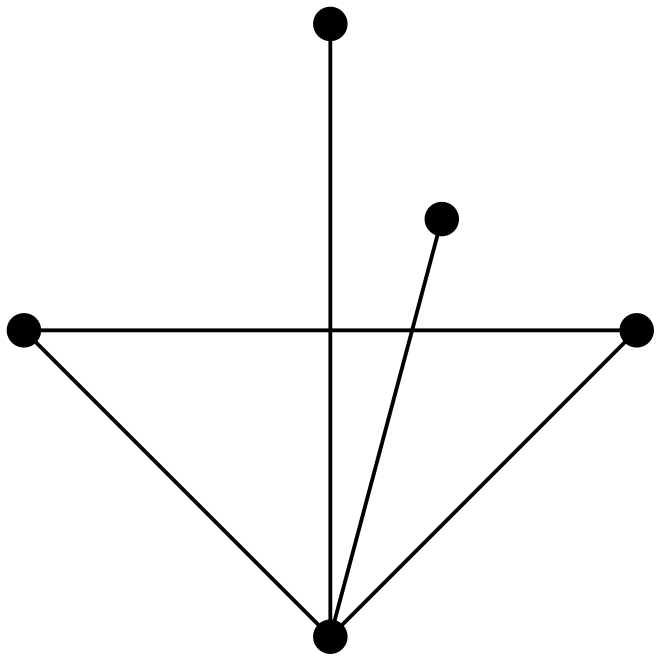
\includegraphics[width=.6\linewidth]{exthgeo}
  \caption{Un thrackle geométrico con cinco vértices.}
  \label{fig:exthgeo}
\end{subfigure}
\caption{Ambas figuras ilustran thrackles definidos sobre el mismo conjunto de
puntos. En los dos casos el thrackle dibujado es máximo.}
\label{fig:exthgeotop}
\end{figure}

Una gráfica (abstracta) $G$ es \emph{thrackleable} si puede ser dibujada en el plano como un thrackle.

Una descomposición por thrackles $D$, de una gráfica geométrica
$\mathsf{G}$, es una colección $D=\{\mathsf{G}_1,\mathsf{G}_2,\dots,\mathsf{G}_k\}$
de subgráficas geométricas que cumple con tres condiciones:
\begin{enumerate}
  \item Cada subgráfica $\mathsf{G}_i$ es un thrackle.
  \item Ninguna subgráfica $\mathsf{G}_i$ contiene vértices aislados.
  \item Cada arista de $\mathsf{G}$ pertenece a exactamente una subgráfica
  $\mathsf{G}_i$ de $D$.
\end{enumerate}

Un thrackle en el que todas sus aristas son segmentos de recta es conocido como
\emph{thrackle geométrico}(\cite{Schaefer2018}). En la
figura~\ref{fig:exthgeotop} presentamos un ejemplo de thrackle y un ejemplo de
thrackle geométrico. En este trabajo nos referimos a los thrackles geométricos
como thrackles ya que solo estudiamos descomposiciones de gráficas con
thrackles geométricos.

Además definimos la intersección entre dos thrackles como sigue:

\begin{definition}{\emph{Intersección de dos thrackles}.} Sea $T_i$ y $T_j$ dos
  thrackles con el mismo número de arista, definimos la intersección de $T_i$ y
  $T_j$ como la intersección de sus conjuntos de aristas correspondientes. En
  otras palabras:
  \[ T_i \cap T_j = E(T_i) \cap E(T_j).\]
\end{definition}

Decimos que dos thrackles $T_i$ y $T_j$ son disjuntos cuando $T_i\cap T_j = \emptyset$. Además, decimos que
un thrackle $T$ es de \emph{tamaño} $k$ si $E(T)=k$.

En este trabajo representamos un thrackle $T$ de tamaño $k$ con una tupla de enteros positivos
$\{e_1,e_2,\dots,e_k\}$ tales que $e_1 < e_2 < \dots < e_k$. Decimos que $T=\{e_1,e_2,\dots,e_k\}$ tiene a
las aristas $e_1,e_2,\dots,e_k$. Esta representación nos permite dar un orden para dos thrackles.

\begin{definition}{\emph{Ordenamiento de dos thrackles}.}
  Sea $T_1 =\{e_1,e_2,\dots,e_{t_1}\}$ y $T_2 =\{f_1,f_2,\dots,f_{t_2}\}$ dos thrackles con tamaño $t_1$ y
  $t_2$ respectivamente. Decimos que $T_1 < T_2$ si y solo si existe $e_i \in T_1$ y $f_i \in T_2$ tal que
  $e_i < f_i$ o bien, si $t_1 > t_2$.
\end{definition}

Para ejemplificar la definición anterior supongamos que $T_1=\{1,3,6,8,12\}$ y que $T_2=\{1,3,6,9,10\}$, en
este caso $T_1 < T_2$ ya que $8 < 9$. Por otro lado, si $T_3=\{1,3,4\}$ tenemos que $T_1 < T_3$ porque
$T_3$ tiene tres aristas y $T_1$ tiene cinco aristas.

Dada una gráfica completa (abstracta) esta puede ser dibujada en el plano
de muchas maneras, solo basta con mover un punto en cualquier dirección
para obtener diferentes dibujos de la misma gráfica completa, de hecho
hay un número no finito de dibujos para una sola gráfica abstracta. Estudiarlos
todos no es posible y por ello necesitamos discretizar el número de
posibles dibujos geométricos para una sola gráfica. El tipo de orden es
una herramienta que otorga un número finito de dibujos combinatoriamente
diferentes para gráficas abstractas.Explicamos este concepto a continuación.

\subsection{Tipo de Orden}

Para entender cómo funciona el tipo de orden de un conjunto de puntos
debemos definir la orientación de una tripleta de puntos.

Tres puntos $(p,q,w)$ en el plano en posición general, pueden tener una
orientación en sentido horario o una orientación en sentido anti-horario.
Decimos que $(p,q,w)$ está orientada en sentido horario si $w$ está a la
derecha del segmento dirigido $\overline{pq}$. Si $w$ está a la izquierda
de dicho segmento entonces $(p,q,w)$ está orientada en sentido anti-horario.
Si la tripleta está orientada en sentido horario asignamos a esa tripleta el
valor $-1$. Si la tripleta está orientada en sentido anti-horario asignamos a
esa tripleta el valor $+1$. En la figura~\ref{fig:triplet} mostramos un ejemplo
de cada orientación posible para una tripleta.
\begin{figure}[htpb]
  \centering
  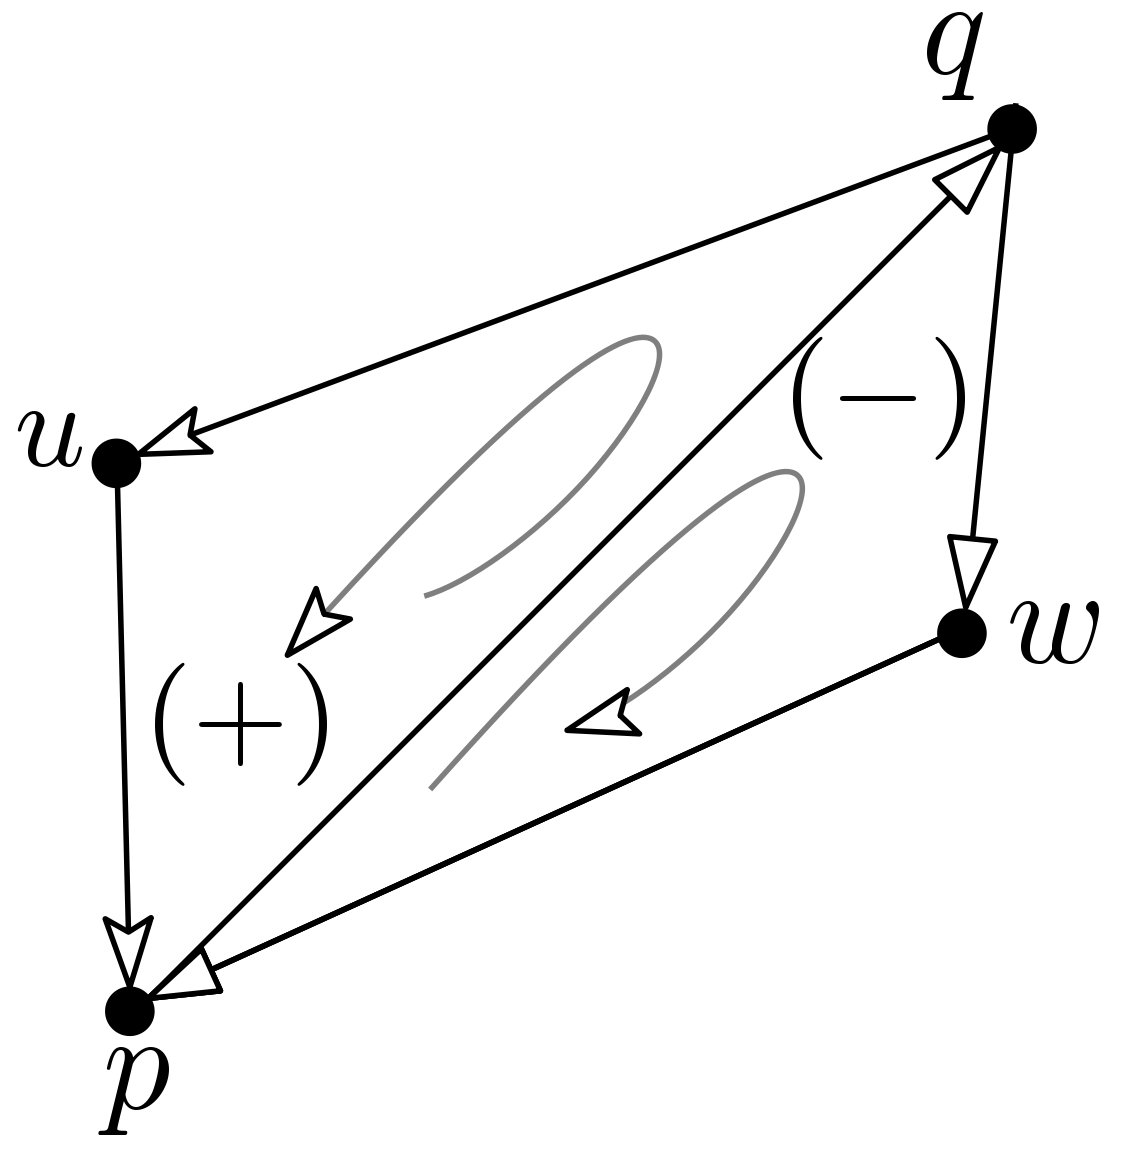
\includegraphics[width=0.30\linewidth]{triplet}
  \caption{Esta figura muestra las posibles orientaciones de una tripleta de
  puntos. La tripleta $\{p,q,w\}$ tiene asignado el valor de $(-1)$ porque $w$
  está orientado en sentido horario con respecto del segmento $\overline{pq}$.
  La tripleta $\{p,q,u\}$ tiene asignado el valor de $(+1)$  porque $u$ está
  orientado en sentido anti-horario con respecto del mismo segmento.}
  \label{fig:triplet}
\end{figure}

Las definiciones siguientes fueron tomadas de~\cite{Aichholzer2002}.
El tipo de orden de un conjunto $S=\{p_1,p_2,\dots,p_n\}$ de puntos en posición
general, es una función que asigna a cada tripleta ordenada
$i,j,k \in \{1,2,\dots,n\}$ la orientación de la tripleta de puntos
$\{p_i,p_j,p_k\}$.

%FALTA DISCUTIR LA RELACIÓN DON DESCOMPOSICIONES DE GRÁFICAS GEOMÉTRICAS.
Decimos que dos conjuntos $S_1$ y $S_2$ son \emph{combinatoriamente
equivalentes} si tienen el mismo tipo de orden de otra forma, si no son
equivalentes decimos que son \emph{combinatoriamente distintos}. Si $S_1$ y
$S_2$ son combinatoriamente equivalentes dos segmentos en $S_1$ se cruzan si y
solo si los segmentos correspondientes en $S_2$ se cruzan. Solo hay una manera
(combinatoriamente equivalente) de acomodar tres puntos,
dos maneras de acomodar cuatro puntos y tres maneras de acomodar cinco puntos.
En la figura~\ref{fig:exotk34} ilustramos los diferentes tipos de orden
para conjuntos de tres y cuatro puntos. En la figura~\ref{fig:exotk5}
presentamos conjuntos combinatoriamente equivalentes de cinco puntos. En la
figura~\ref{fig:ot5} mostramos los diferentes tipos de orden para un conjunto
de cinco puntos.

\begin{figure}[htpb]
  \centering
  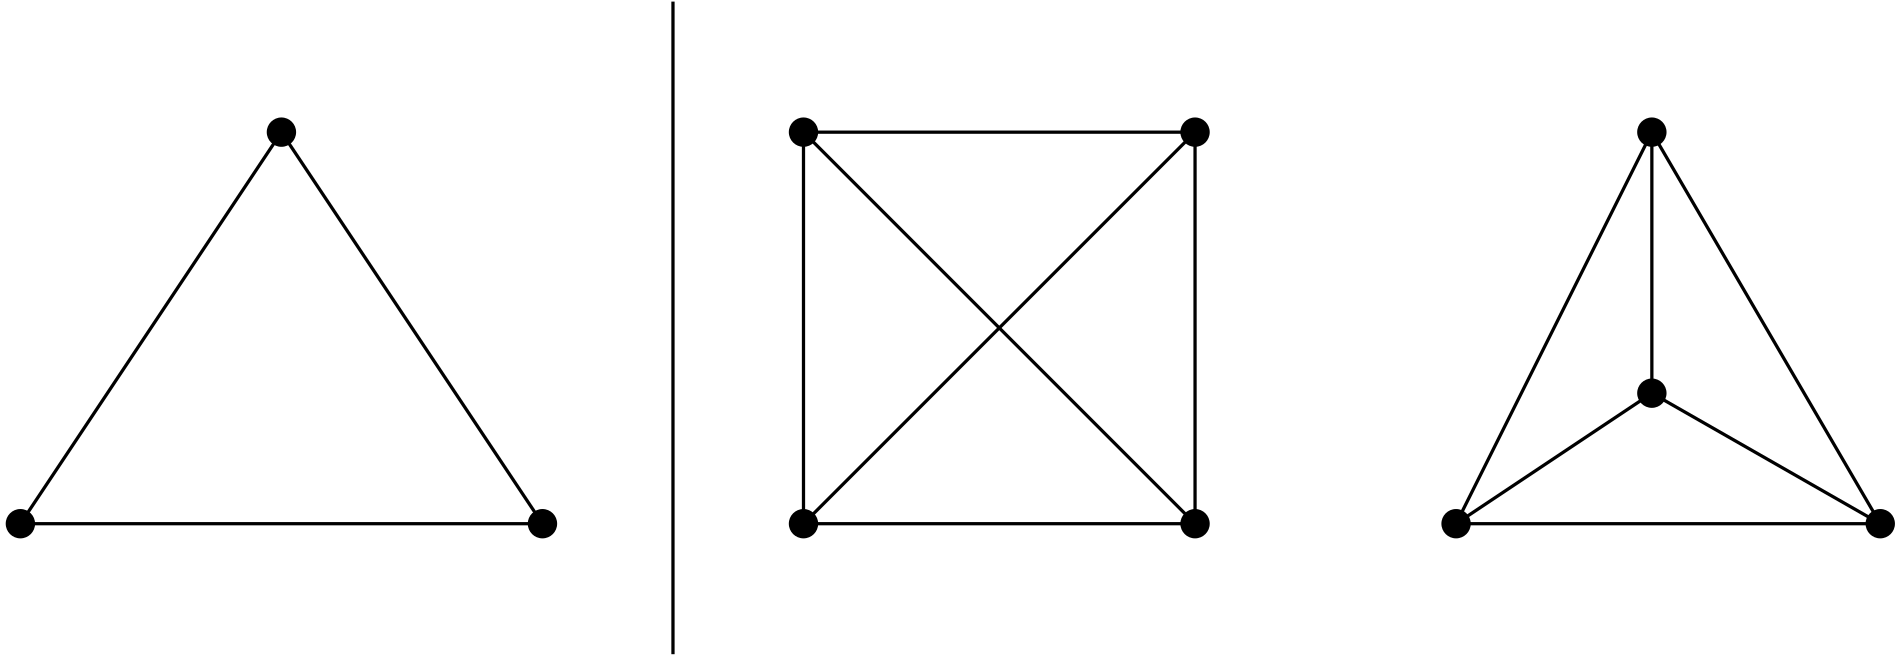
\includegraphics[width=0.8\linewidth]{exot34}
  \caption{Las diferentes maneras combinatoriamente diferentes
  de acomodar 3 y 4 puntos.}
  \label{fig:exotk34}
\end{figure}
\begin{figure}[htpb]
  \centering
  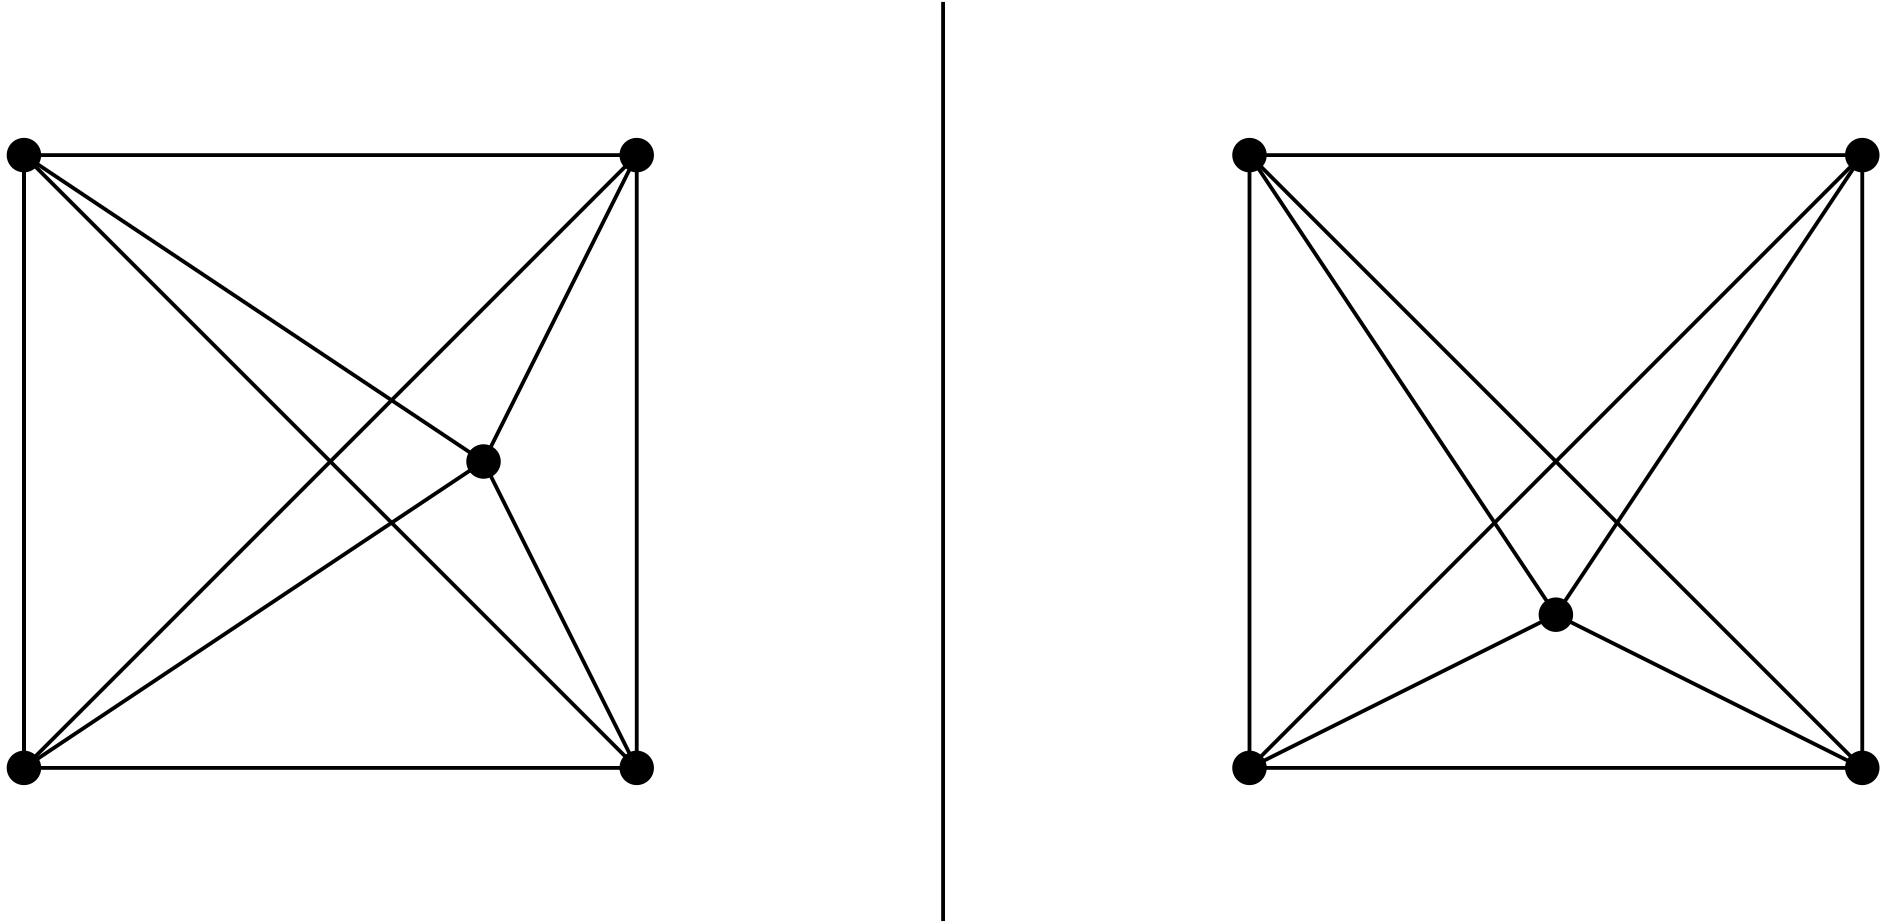
\includegraphics[width=0.8\linewidth]{exotk5}
  \caption{Estos dos conjuntos de puntos tienen el mismo tipo de orden.
  Observe que el valor de cada una de las tripletas del dibujo
  que está a la izquierda es igual al valor de las tripletas del
  dibujo a la derecha.}
  \label{fig:exotk5}
\end{figure}
\begin{figure}[htpb]
  \centering
  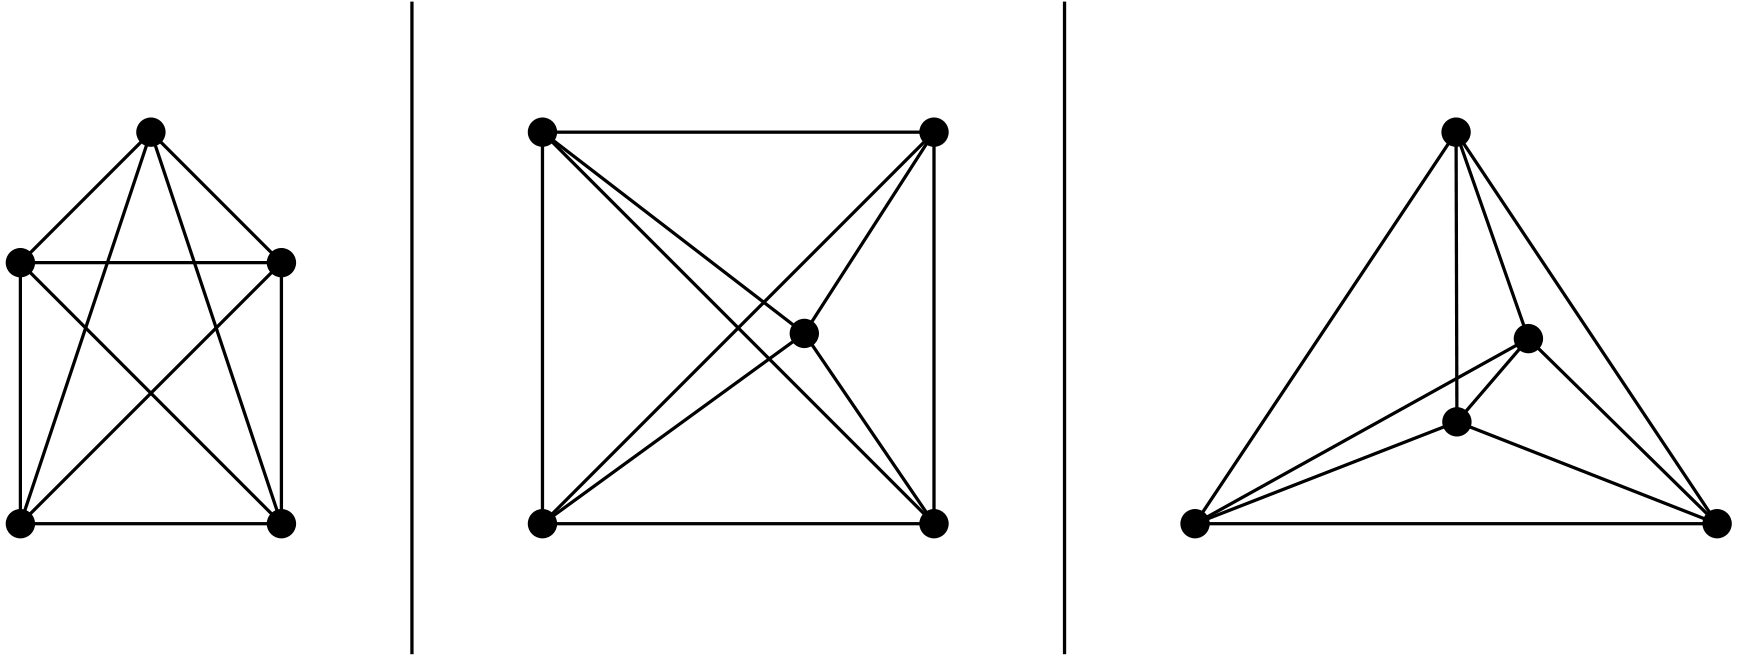
\includegraphics[width=0.8\linewidth]{ot5}
  \caption{Las tres maneras diferentes de distribuir 5 puntos en el plano.
  Cualquier otra configuración es equivalente a alguna de estas tres
  configuraciones.}
  \label{fig:ot5}
\end{figure}

%%ILUSTRAR ESTE PÁRRAFO CON UN EJEMPLO DE N=6
No es trivial enumerar o contar los conjuntos combinatoriamente diferentes, por
ejemplo, dados $n$ puntos podemos colocarlos en posición convexa y obtener el
primer tipo de orden para $n$ puntos, luego podemos colocar $n-1$ puntos en
posición convexa y un punto dentro del $(n-1)$-ágono y evaluar de cuántas
maneras combinatoriamente distintas es posible colocar un punto dentro del
polígono. Posteriormente podemos ver que pasa con $n-2$ puntos en posición
convexa y dos dentro del $(n-2)-$ágono y así sucesivamente hasta que tengamos 3
puntos en posición convexa y $n-(n-3)$ dentro del triángulo. En la figura
~\ref{fig:exotk6} explicamos una parte de este proceso. Usando una técnica
parecida se sabe que para $n=10$ hay más de 14 millones de tipos de orden.
\begin{figure}[htpb]
  \centering
  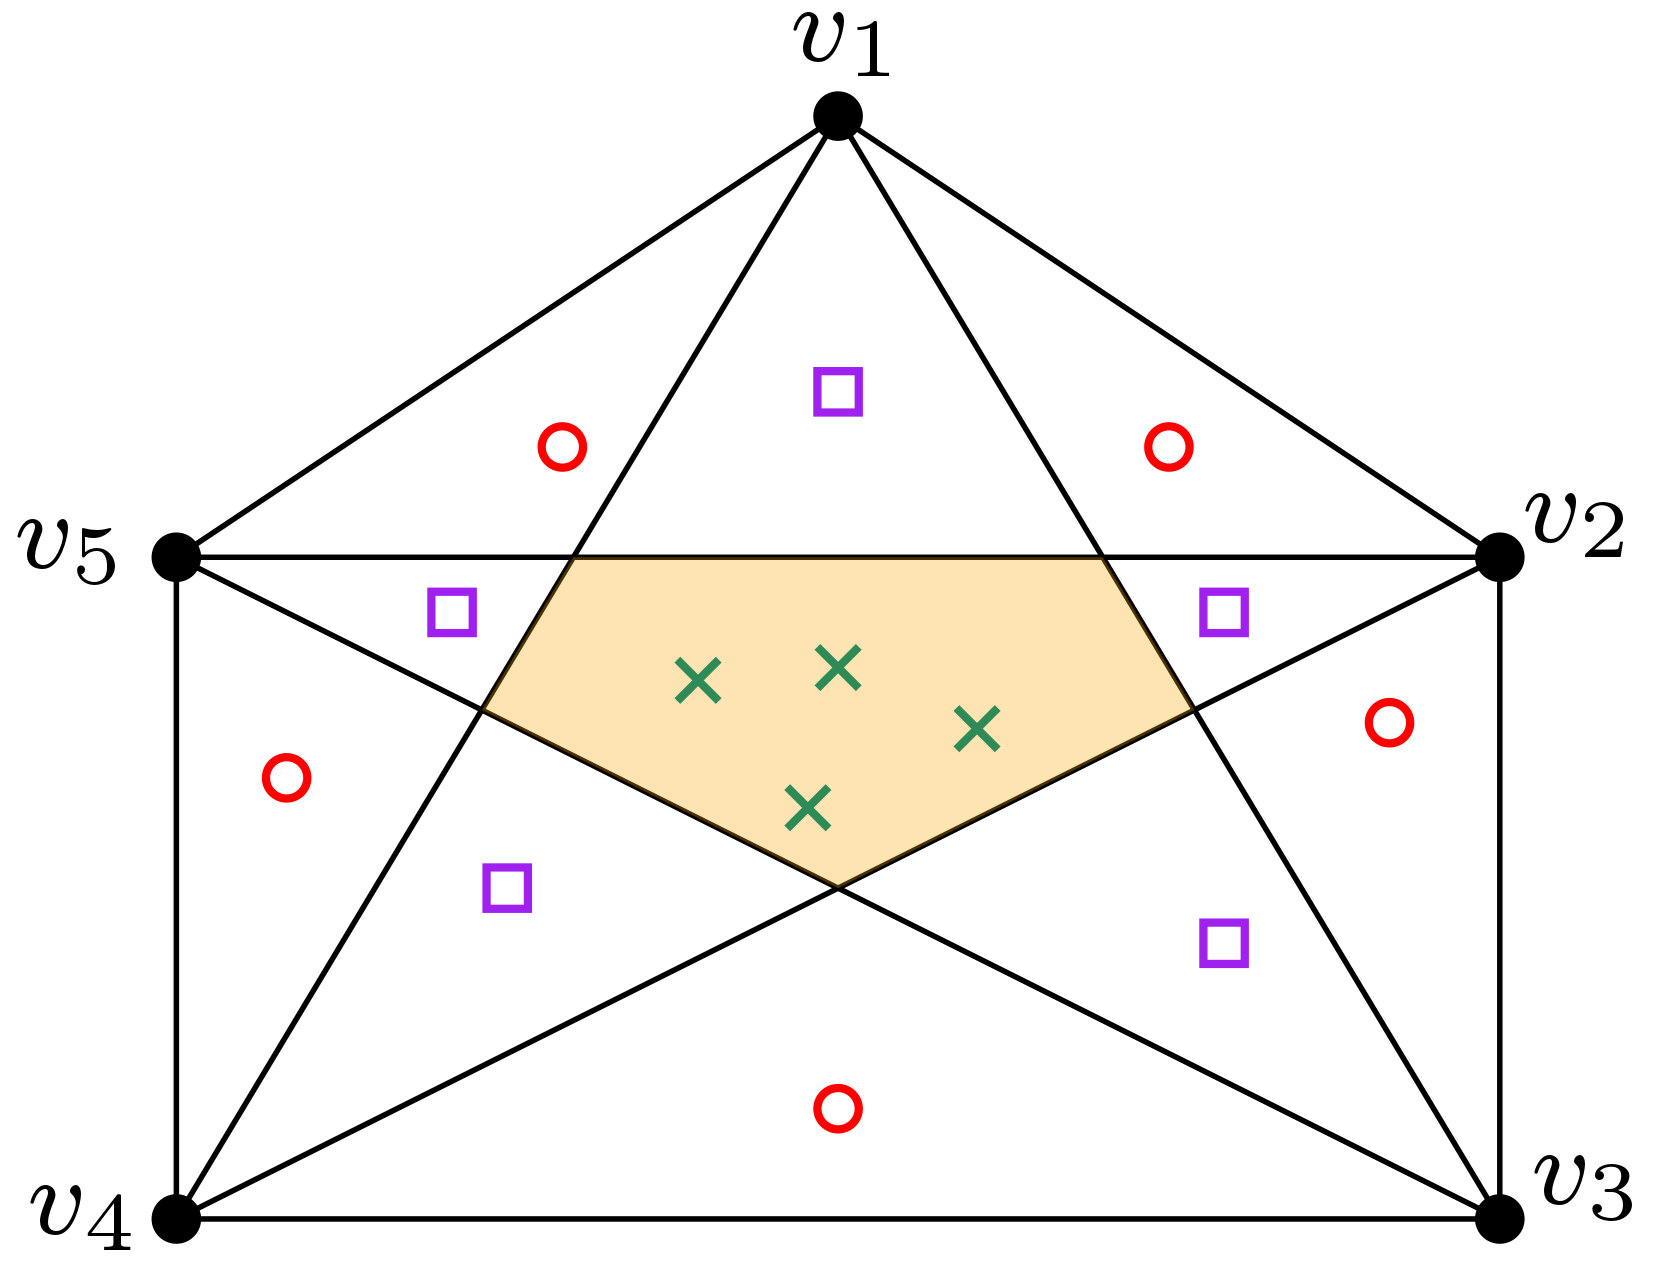
\includegraphics[width=0.5\linewidth]{exotk6}
  \caption{La figura ilustra las diferentes maneras de colocar un punto
  dentro de un pentágono, para formar un conjunto de 6 puntos en total.
  Hay al menos 3 formas diferentes de colocar dicho punto, 1) es posible
  ponerlo dentro del pentágono pero fuera del polígono en forma de estrella
  inducido por las aristas del ciclo interior. 2) Es posible ponerlo
  dentro de uno de los "picos`` del polígono en forma de estrella y 3)
  es posible ubicarlo en el área rellena. Los puntos de 1) están
  representados con un círculo sin rellenar, los puntos de 2) con un cuadrado
  y los puntos de 3) con una cruz. La razón por la que existe más de una
  ocurrencia de un mismo tipo de punto es porque existe una equivalencia en la
  etiquetación de los vértices tales que los cruces se preservan.}
  \label{fig:exotk6}
\end{figure}
En el trabajo de~\cite{Aichholzer2002} se ofrece una base de datos que contiene
los conjuntos combinatoriamente diferentes para toda $3\leq n\leq 10$. En la
tabla~\ref{tab:ots} se presenta el número de conjuntos diferentes para cada $n$
y el tamaño en bytes de la base de datos.

En este trabajo buscamos descomposiciones de gráficas geométricas completas en
thrackles. Como se mencionó antes, un conjunto de $n$ puntos en posición general
induce una gráfica completa de $n$ vértices en el plano. Nosotros analizamos
cada tipo de orden para cada $n\leq 10$ induciendo la gráfica completa de $n$
vértices. Después examinamos sus thrackles y luego buscamos una descomposición.
Cuando buscamos una descomposición que minimiza el número de thrackles
utilizados estamos buscando el anti-thickness de la gráfica. Dicho concepto
será explicado formalmente en seguida.
\begin{table}[ht]
  \centering
  \begin{tabular}{|c|c|r|}
  \hline
  $n$ & Número de tipos de orden & Tamaño (bytes)   \\ \hline
  3     & 1                   & 6       \\ \hline
  4     & 2                   & 16      \\ \hline
  5     & 3                   & 30      \\ \hline
  6     & 16                  & 192     \\ \hline
  7     & 135                 & 1890    \\ \hline
  8     & 3315                & 53040   \\ \hline
  9     & 158817              &	5 717 412   \\\hline
  10    & 14309547            & 572 381 880 \\ \hline
  \end{tabular}
  \caption{Tipos de orden para cada $n\leq10$.}
  \label{tab:ots}
\end{table}

\section{Anti-thickness y anti-thickness geométrico} \label{secc:anti-thickness}
Las siguientes definiciones fueron tomadas de~\cite{Dujmovic2017}.
\begin{definition}{\emph{Anti-thickness de una gráfica.}}
  El anti-thickness de una gráfica $G$ es el entero $k$ más pequeño tal que
  existe una partición de $E(G)$, de tamaño $k$, en la que cada elemento de la
  partición es una gráfica thrackleable.
\end{definition}
La figura~\ref{fig:exantithickness} ilustra un ejemplo del anti-thickness de
$K_5$.
\begin{figure}[htpb]
  \centering
  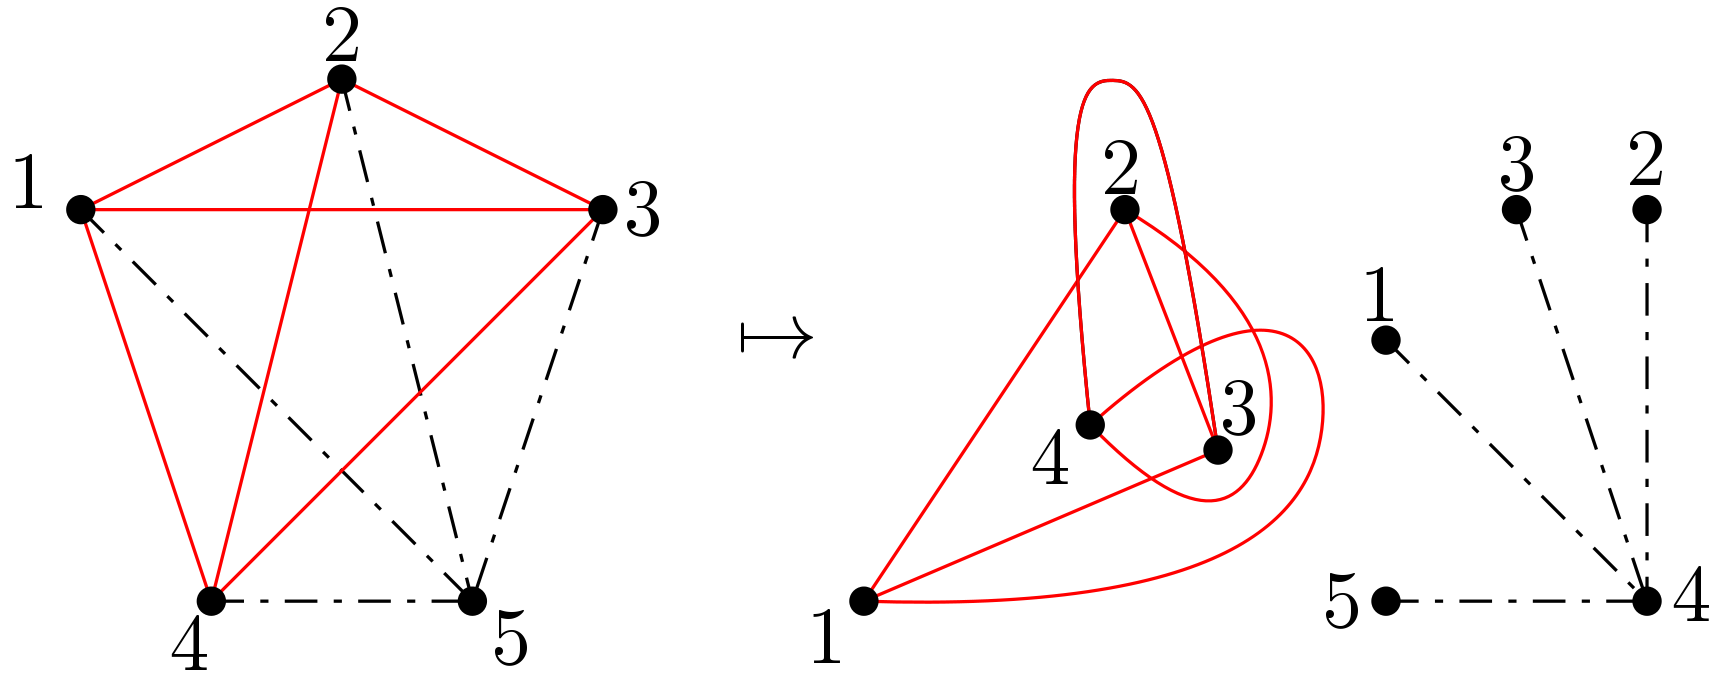
\includegraphics[width=0.7\linewidth]{exantithickness}
  \caption{La figura muestra a $K_5$ a la izquierda y a la derecha dos thrackles
  cuya unión es $K_5$. Consideremos las aristas de la gráfica completa inducida por los vértices $1,2,3,4$,
  estas aristas inducen un thrackle mientras que las aristas con un extremo en el vértice $5$ inducen otro thrackle.
  El anti-thickness de $K_5$ es precisamente igual a dos. Este resultado se discute en el capítulo de resultados.}
  \label{fig:exantithickness}
\end{figure}

Cuando deseamos que los thrackles usados en la descomposición de la gráfica sean
geométricos, entonces podemos definir el anti-thickness geométrico como sigue.
\begin{definition}{\emph{Anti-thickness geométrico de una gráfica.}}
El anti-thickness geométrico de una gráfica $G$ es el entero $k$ más pequeño
tal que existe un dibujo $\mathsf{G}$ de $G$ para el cual hay una partición de
$E(\mathsf{G})$, de tamaño $k$, en la que cada elemento de la partición induce
un thrackle.
\end{definition}
Nótese que en la partición que realiza el anti-thickness de la gráfica, cada
elemento de la partición tiene uno o más dibujos, mientras que en la partición
que realiza el anti-thickness geométrico de la gráfica, cada elemento es una
subgráfica geométrica del dibujo original.

En la figura~\ref{fig:exantithicknessgeo} damos un ejemplo del anti-thickness
geométrico de $K_5$.
\begin{figure}[htpb]
  \centering
  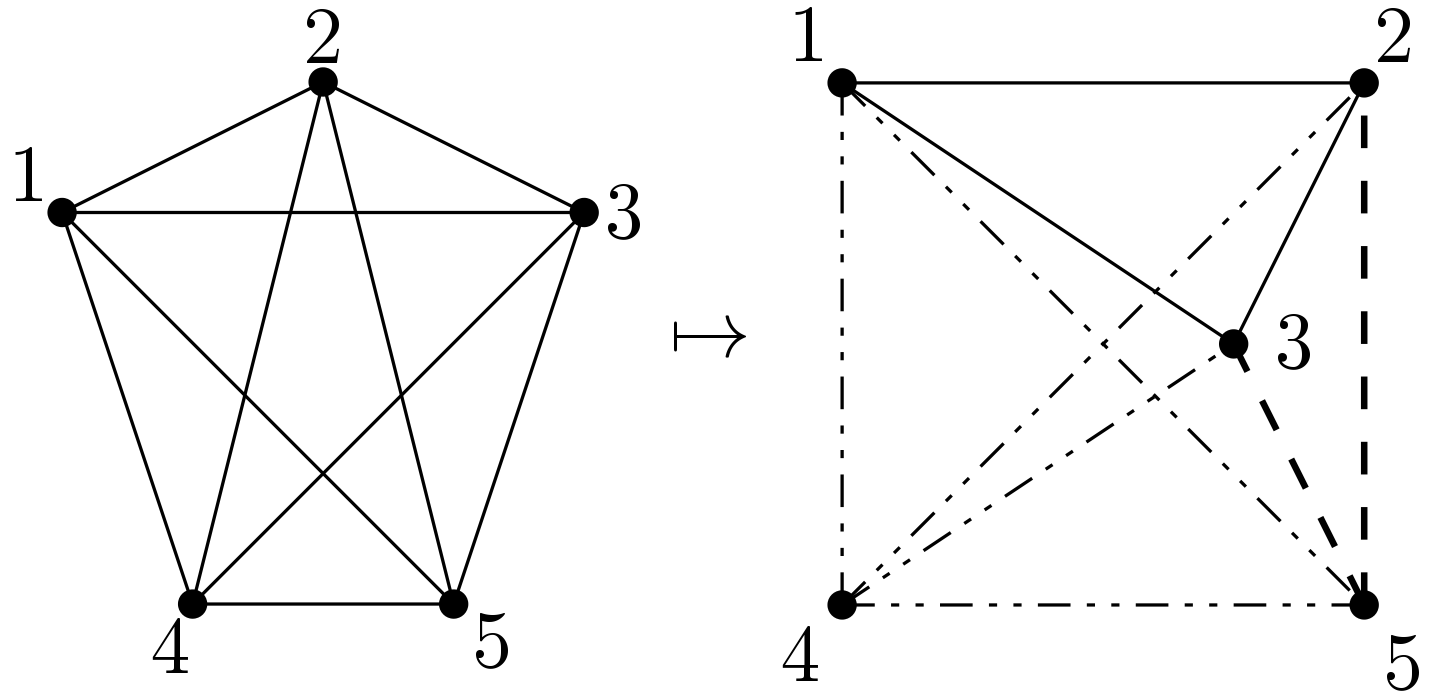
\includegraphics[width=0.6\linewidth]{exantithicknessgeo}
  \caption{En esta figura podemos observar una descomposición de $K_5$ en 3
  thrackles geométricos. Esta descomposición se muestra en la figura del lado
  derecho, cada thrackle está dibujado con diferentes patrones de línea. El
  anti-thickness geométrico de $K_5$ es exactamente tres, esto es demostrado en
  la sección de resultados.} %FALTA CITAR <<<<<<<<<<<<<<<<<<<<<<<
  \label{fig:exantithicknessgeo}
\end{figure}

También es posible definir el anti-thickness de una gráfica geométrica como sigue:
\begin{definition}{\emph{Anti-thickness de una gráfica geométrica}}
  \label{definicion:at_dibujo}
  El anti-thickness $At_g(\mathsf{G})$ de una gráfica geométrica $\mathsf{G}$
  es el entero $k$ más pequeño tal que existe una partición de $E(\mathsf{G})$, de tamaño $k$, en la que cada elemento de la partición es un thrackle.
\end{definition}

Dar una descomposición de una gráfica en thrackles es equivalente a encontrar
conjuntos independientes de aristas que comparten ciertas propiedades. A su vez,
encontrar los conjuntos independientes de una gráfica está relacionado a
encontrar el \emph{número cromático} de una gráfica (abstracta). Discutimos
esto en la siguiente sección.

\section{Número cromático}
Las siguientes definiciones fueron tomadas de~\cite{Chartrand2008}.

Una \emph{coloración propia} de los vértices de una gráfica $G$ es la asignación
de colores a los vértices de $G$ tal que cada vértice tiene un solo color
asignado y dos vértices adyacentes tienen diferentes colores.
Un color puede ser un color como rojo, verde, amarillo, etc. cuando el número
de colores a usar es pequeño, de otra forma se usan enteros $1,2,\dots,k$
para algún entero positivo $k$ para representar los colores. Si la coloración
propia usa $k$ colores diferentes decimos que tenemos una \emph{k-coloración}
de la gráfica $G$. Dada una $k$-coloración de una gráfica $G$, si $V_i$ es el
conjunto de vértices de $G$ que tienen el color $i$ asignado, llamamos a $V_i$
una \emph{clase cromática} de $G$. El conjunto $\{V_1,V_2,\dots,V_k\}$ genera
una partición en conjuntos independientes de los vértices de $G$.

Una gráfica $G$ es \emph{k-colorable} si existe una coloración propia de $G$ de
tamaño $k$. El entero positivo $k$ más pequeño para el cual $G$ es
$k$-colorable recibe el nombre de \emph{número cromático} de $G$. Lo denotamos
como $\chi(G)$.

% Si consideramos cualquier partición de $V(G)$, el número cromático $\chi(G)$ de $G$ es la
% cardinalidad más pequeña posible de dicha partición.
% El número cromático
% de $G$ es el mínimo número de conjuntos independientes que pueden existir en una partición
% de $V(G)$.

La figura~\ref{fig:excoloring} muestra un ejemplo de una coloración propia de
una gráfica $G$. En este ejemplo ilustramos cada clase cromática dibujando los
vértices con diferentes colores representados por una cruz, un círculo y un
cuadrado.
\begin{figure}[htpb]
  \centering
  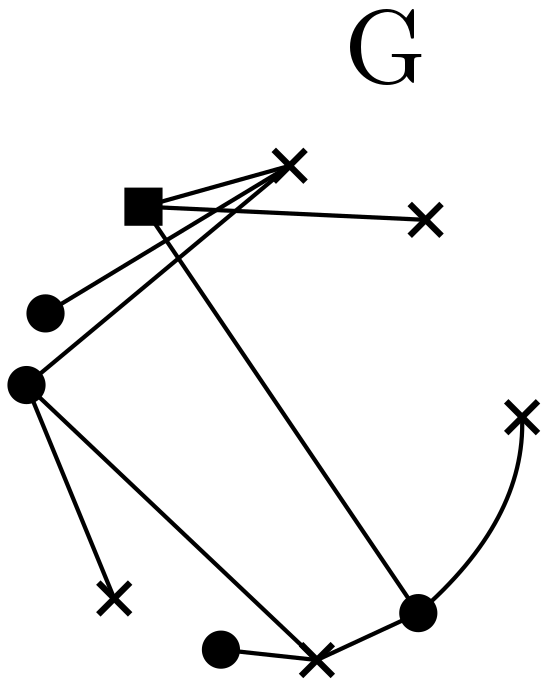
\includegraphics[width=0.25\linewidth]{excoloring}
  \caption{Una coloración propia de una gráfica $G$. Esta coloración es de
  tamaño 3, por lo tanto decimos que es una 3-coloración de $G$. Para esta
  gráfica en particular no existe una coloración más pequeña, por lo que su
  número cromático es 3. Nótese que los conjuntos independientes son formados
  por vértices que tienen el mismo color asignado y no son adyacentes entre sí.}
  \label{fig:excoloring}
\end{figure}
%%%%% FALTA CONECTAR CON LA DESCOMPOSICIÓN
Si tenemos una descomposición en $k$ thrackles de una gráfica geométrica y
asignamos uno de $k$ colores a cada thrackle de la descomposición de tal
manera que no existan dos thrackles del mismo color y si además minimizamos
el valor de $k$ entonces $k$ es el anti-thickness de la gráfica geométrica dada.
Esta idea ha sido utilizada para encontrar el anti-thickness de una gráfica
geométrica cuyos vértices están en posición convexa. Detallamos este concepto en
la siguiente sección.

%%RESUMEN DE CAPITULO
En este capítulo explicamos los conceptos necesarios para entender el trabajo
realizado en esta tesis. Empezamos hablando de gráficas abstractas y después de
su representación en el plano usando aristas que son curvas y usando aristas
que son segmentos de recta a las cuales llamamos gráficas geométricas.
Continuamos definiendo un tipo especial de gráfica geométrica en la cual cada
par de aristas se intersecta, este tipo de gráfica geométrica recibe el nombre
de thrackle. Luego explicamos el tipo de orden como herramienta para
discretizar el número de dibujos posibles de una gráfica en el plano.
Después hablamos del anti-thickness geométrico de una gráfica como el mínimo
número de thrackles que existen en una descomposición para todos los dibujos de
una gráfica. Finalmente mencionamos el número cromático como el mínimo número
de conjuntos independientes que existen en una partición de los vértices de una
gráfica. Este último punto es de importancia para el siguiente capítulo pues
explicamos cómo el problema de encontrar el anti-thickness geométrico de una
gráfica puede ser visto como un problema de encontrar el número cromático.
Además hablaremos de cuáles son los aportes más recientes acerca del problema
del anti-thickness geométrico.
